% Options for packages loaded elsewhere
\PassOptionsToPackage{unicode}{hyperref}
\PassOptionsToPackage{hyphens}{url}
%
\documentclass[
]{article}
\usepackage{amsmath,amssymb}
\usepackage{lmodern}
\usepackage{iftex}
\ifPDFTeX
  \usepackage[T1]{fontenc}
  \usepackage[utf8]{inputenc}
  \usepackage{textcomp} % provide euro and other symbols
\else % if luatex or xetex
  \usepackage{unicode-math}
  \defaultfontfeatures{Scale=MatchLowercase}
  \defaultfontfeatures[\rmfamily]{Ligatures=TeX,Scale=1}
\fi
% Use upquote if available, for straight quotes in verbatim environments
\IfFileExists{upquote.sty}{\usepackage{upquote}}{}
\IfFileExists{microtype.sty}{% use microtype if available
  \usepackage[]{microtype}
  \UseMicrotypeSet[protrusion]{basicmath} % disable protrusion for tt fonts
}{}
\makeatletter
\@ifundefined{KOMAClassName}{% if non-KOMA class
  \IfFileExists{parskip.sty}{%
    \usepackage{parskip}
  }{% else
    \setlength{\parindent}{0pt}
    \setlength{\parskip}{6pt plus 2pt minus 1pt}}
}{% if KOMA class
  \KOMAoptions{parskip=half}}
\makeatother
\usepackage{xcolor}
\usepackage{longtable,booktabs,array}
\usepackage{multirow}
\usepackage{calc} % for calculating minipage widths
% Correct order of tables after \paragraph or \subparagraph
\usepackage{etoolbox}
\makeatletter
\patchcmd\longtable{\par}{\if@noskipsec\mbox{}\fi\par}{}{}
\makeatother
% Allow footnotes in longtable head/foot
\IfFileExists{footnotehyper.sty}{\usepackage{footnotehyper}}{\usepackage{footnote}}
\makesavenoteenv{longtable}
\usepackage{graphicx}
\makeatletter
\def\maxwidth{\ifdim\Gin@nat@width>\linewidth\linewidth\else\Gin@nat@width\fi}
\def\maxheight{\ifdim\Gin@nat@height>\textheight\textheight\else\Gin@nat@height\fi}
\makeatother
% Scale images if necessary, so that they will not overflow the page
% margins by default, and it is still possible to overwrite the defaults
% using explicit options in \includegraphics[width, height, ...]{}
\setkeys{Gin}{width=\maxwidth,height=\maxheight,keepaspectratio}
% Set default figure placement to htbp
\makeatletter
\def\fps@figure{htbp}
\makeatother
\usepackage[normalem]{ulem}
\setlength{\emergencystretch}{3em} % prevent overfull lines
\providecommand{\tightlist}{%
  \setlength{\itemsep}{0pt}\setlength{\parskip}{0pt}}
\setcounter{secnumdepth}{-\maxdimen} % remove section numbering
\ifLuaTeX
  \usepackage{selnolig}  % disable illegal ligatures
\fi
\IfFileExists{bookmark.sty}{\usepackage{bookmark}}{\usepackage{hyperref}}
\IfFileExists{xurl.sty}{\usepackage{xurl}}{} % add URL line breaks if available
\urlstyle{same} % disable monospaced font for URLs
\hypersetup{
  hidelinks,
  pdfcreator={LaTeX via pandoc}}

\author{}
\date{}

\begin{document}

\begin{quote}
An Overview of Finding Maxima and Minima of Functions
\end{quote}

Prepared by {[}Your Name{]}

November 1, 2024

\begin{quote}
\textbf{Contents}
\end{quote}

\begin{longtable}[]{@{}
  >{\raggedright\arraybackslash}p{(\columnwidth - 6\tabcolsep) * \real{0.2500}}
  >{\raggedright\arraybackslash}p{(\columnwidth - 6\tabcolsep) * \real{0.2500}}
  >{\raggedright\arraybackslash}p{(\columnwidth - 6\tabcolsep) * \real{0.2500}}
  >{\raggedright\arraybackslash}p{(\columnwidth - 6\tabcolsep) * \real{0.2500}}@{}}
\toprule()
\begin{minipage}[b]{\linewidth}\raggedright
\textbf{1}
\end{minipage} &
\multicolumn{2}{>{\raggedright\arraybackslash}p{(\columnwidth - 6\tabcolsep) * \real{0.5000} + 2\tabcolsep}}{%
\begin{minipage}[b]{\linewidth}\raggedright
\begin{quote}
\textbf{Introduction}
\end{quote}
\end{minipage}} & \begin{minipage}[b]{\linewidth}\raggedright
\begin{quote}
\textbf{2}
\end{quote}
\end{minipage} \\
\midrule()
\endhead
\textbf{2} &
\multicolumn{2}{>{\raggedright\arraybackslash}p{(\columnwidth - 6\tabcolsep) * \real{0.5000} + 2\tabcolsep}}{%
\begin{minipage}[t]{\linewidth}\raggedright
\begin{quote}
\textbf{Mathematical Formulation}
\end{quote}
\end{minipage}} & \begin{minipage}[t]{\linewidth}\raggedright
\begin{quote}
\textbf{3}
\end{quote}
\end{minipage} \\
\multirow{2}{*}{\textbf{3}} & \textbf{Example:} & \textbf{Finding the
Maxima and Minima of a Quadratic} &
\multirow{2}{*}{\begin{minipage}[t]{\linewidth}\raggedright
\begin{quote}
\textbf{4}
\end{quote}
\end{minipage}} \\
&
\multicolumn{2}{>{\raggedright\arraybackslash}p{(\columnwidth - 6\tabcolsep) * \real{0.5000} + 2\tabcolsep}}{%
\begin{minipage}[t]{\linewidth}\raggedright
\begin{quote}
\textbf{Function}
\end{quote}
\end{minipage}} \\
\bottomrule()
\end{longtable}

1

\begin{quote}
\textbf{1 Introduction}

Understanding how to find the maxima and minima of functions is a key
concept in \emph{calculus}. It helps in identifying the highest or
lowest points on a graph, which can have various applications in
physics, economics, and optimization problems.
\end{quote}

2

\begin{quote}
\textbf{2 Mathematical Formulation}\\
To find the \textbf{maxima} or \textbf{minima} of a function
\emph{f}(\emph{x}), we start by finding its first
\end{quote}

\begin{longtable}[]{@{}
  >{\raggedright\arraybackslash}p{(\columnwidth - 4\tabcolsep) * \real{0.3333}}
  >{\raggedright\arraybackslash}p{(\columnwidth - 4\tabcolsep) * \real{0.3333}}
  >{\raggedright\arraybackslash}p{(\columnwidth - 4\tabcolsep) * \real{0.3333}}@{}}
\toprule()
\begin{minipage}[b]{\linewidth}\raggedright
derivative:
\end{minipage} & \begin{minipage}[b]{\linewidth}\raggedright
\begin{quote}
\emph{f′}(\emph{x}) = Derivative of \emph{f}(\emph{x})\emph{.}
\end{quote}
\end{minipage} & \begin{minipage}[b]{\linewidth}\raggedright
(1)
\end{minipage} \\
\midrule()
\endhead
\bottomrule()
\end{longtable}

\begin{quote}
Next, we find the critical points by solving:\\
\emph{f′}(\emph{x}) = 0\emph{.} (2)

The second derivative test is used to determine whether a critical point
is a maximum or minimum:\\
If \emph{f′′}(\emph{x}) \emph{\textgreater{}} 0\emph{,} then it is a
minimum. If \emph{f′′}(\emph{x}) \emph{\textless{}} 0\emph{,} then it is
a maximum. (3)
\end{quote}

3

\begin{quote}
\textbf{3 Example: Finding the Maxima and Minima}

\textbf{of a Quadratic Function}
\end{quote}

Consider the function \emph{f}(\emph{x}) = \emph{−x}2+ 4\emph{x −}3. We
first calculate the derivative and find the critical points.

\begin{quote}
The \uline{first derivativ}e is:\\
\emph{f′}(\emph{x}) = \emph{−}2\emph{x} + 4\emph{.} (4)

Solving for \emph{f′}(\emph{x}) = 0:

\emph{−}2\emph{x} + 4 = 0 =\emph{⇒x} = 2\emph{.} (5)

The second derivative is:\\
\emph{f′′}(\emph{x}) = \emph{−}2\emph{.} (6)

Since \emph{f′′}(2) \emph{\textless{}} 0, \emph{x} = 2 is a maximum
point.
\end{quote}

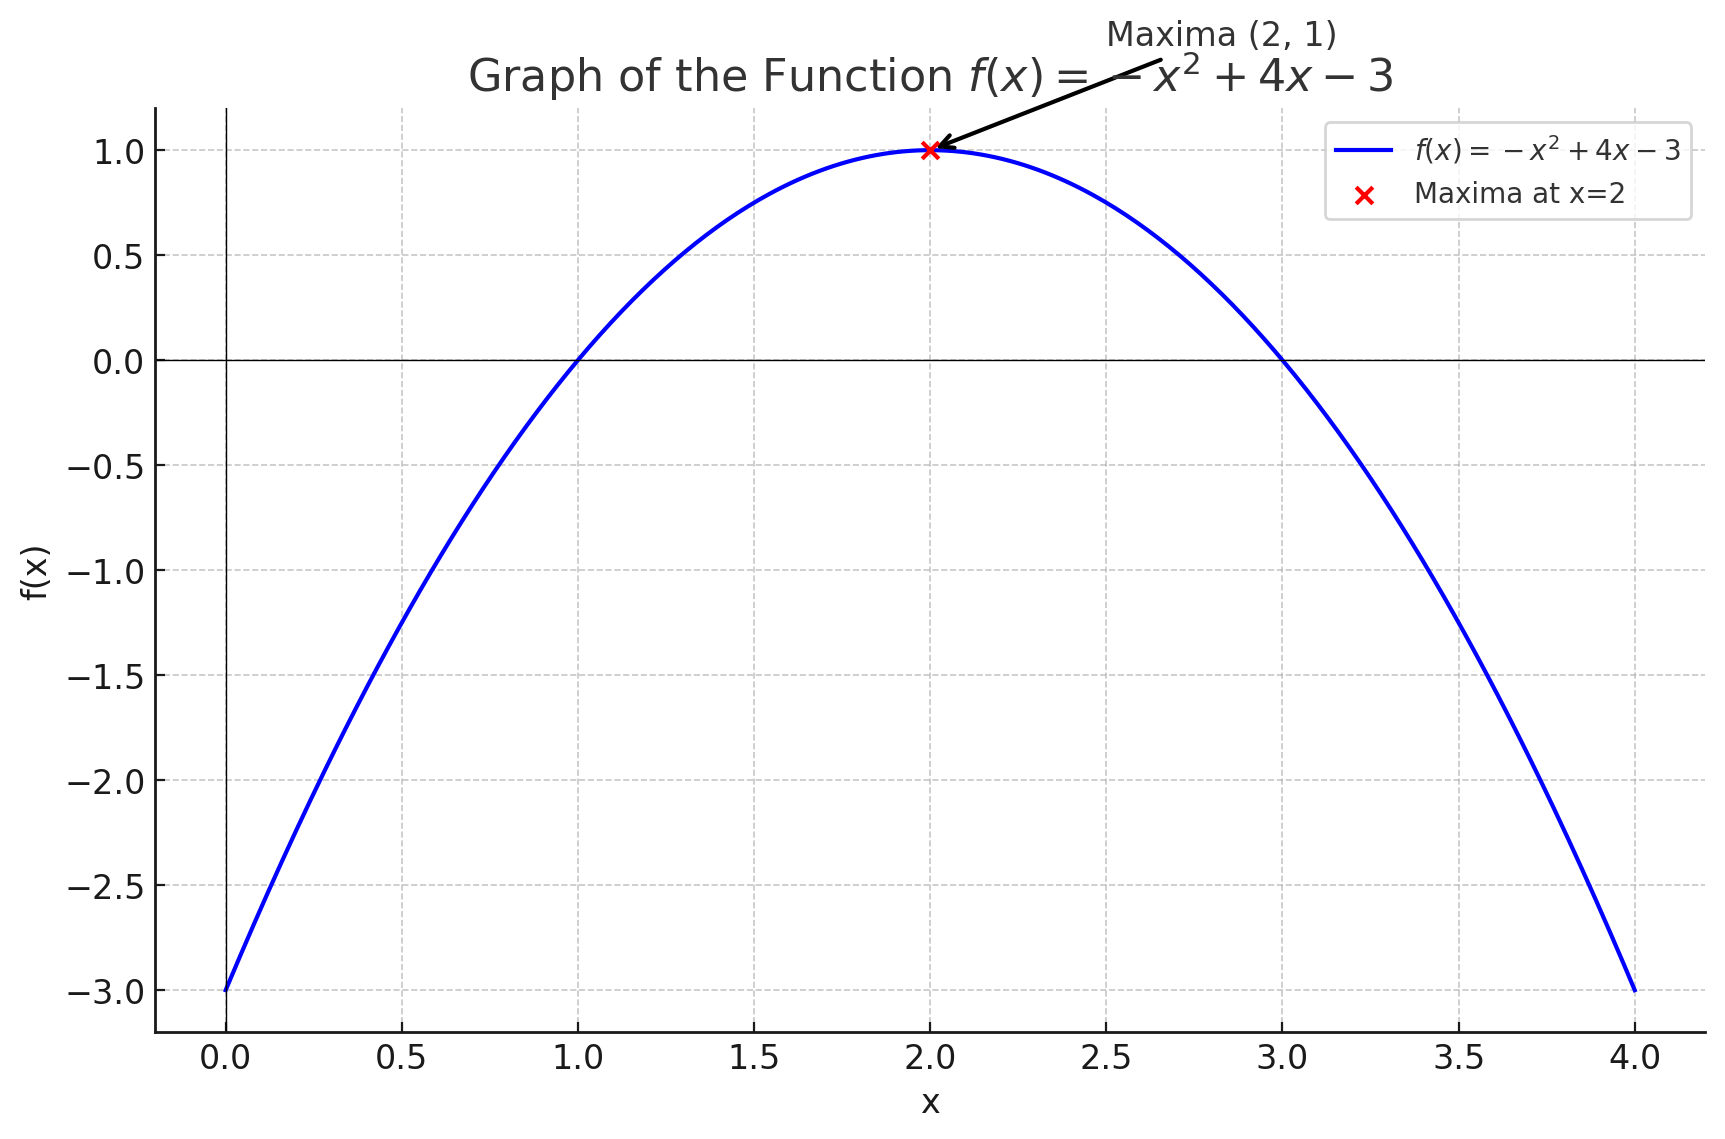
\includegraphics[width=3.34167in,height=2.20694in]{vertopal_39df2c06cf474894b729a41f6de4a54f/media/image1.png}

Figure 1: Graph showing the maxima of the function \emph{f}(\emph{x}) =
\emph{−x}2+ 4\emph{x −}3.

\begin{longtable}[]{@{}
  >{\raggedright\arraybackslash}p{(\columnwidth - 2\tabcolsep) * \real{0.5000}}
  >{\raggedright\arraybackslash}p{(\columnwidth - 2\tabcolsep) * \real{0.5000}}@{}}
\toprule()
\begin{minipage}[b]{\linewidth}\raggedright
\textbf{x}
\end{minipage} & \begin{minipage}[b]{\linewidth}\raggedright
\textbf{f(x)}
\end{minipage} \\
\midrule()
\endhead
\begin{minipage}[t]{\linewidth}\raggedright
\begin{quote}
1\\
2\\
3
\end{quote}\strut
\end{minipage} & \begin{minipage}[t]{\linewidth}\raggedright
\begin{quote}
0\\
1\\
0
\end{quote}\strut
\end{minipage} \\
\bottomrule()
\end{longtable}

Table 1: Values of \emph{f}(\emph{x}) at different points

\begin{quote}
As we can see in Figure 1 and Table 1, the maximum value occurs at
\emph{x} = 2.
\end{quote}

4

\end{document}
